\begin{center}
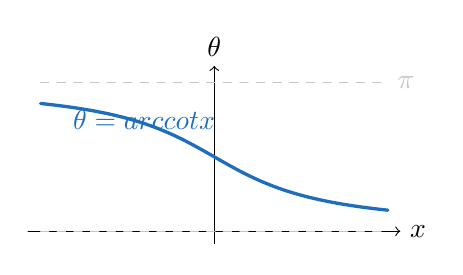
\begin{tikzpicture}[scale=1.05, line cap=round, line join=round]
  \definecolor{trigblue}{RGB}{30,110,190}
  \draw[->] (-2.25,0)--(2.25,0) node[right] {$x$};
  \draw[->] (0,-0.15)--(0,2.0) node[above] {$\theta$};
  \draw[gray!45,dashed] (-2.1,1.8)--(2.1,1.8) node[right] {$\pi$};
  \draw[gray!45,dashed] (-2.1,0)--(2.1,0);
  \draw[very thick,trigblue,domain=-2.1:2.1,samples=90]
    plot ({\x},{0.9+0.9*(-atan(\x)/90)});
  \node[trigblue] at (-0.85,1.35) {$\theta=\operatorname{arccot} x$};
\end{tikzpicture}
\end{center}


\begin{definitionbox}{Definition}
\begin{definition}[Inverse cotangent]
\label{def:inverse-cotangent}
The \emph{inverse cotangent} function is the inverse of cotangent after
cotangent is restricted to the interval $(0,\pi)$. It is denoted by $\operatorname{arccot}$
or $\cot^{-1}$ and has domain $\mathbb{R}$ and range $(0,\pi)$.
\[
  \operatorname{arccot} x=\theta
  \quad\Longleftrightarrow\quad
  \cot\theta=x
  \quad\text{and}\quad
  0<\theta<\pi.
\]
\end{definition}
\end{definitionbox}
\begin{remark*}[Domain and range]
The cotangent function has domain
$\mathbb{R}\setminus\{k\pi:k\in\mathbb{Z}\}$ and range $\mathbb{R}$. The
inverse cotangent function reverses the principal restricted cotangent
function, so its domain is $\mathbb{R}$ and its range is $(0,\pi)$.
\end{remark*}
\begin{dependencies}
\begin{itemize}
  \item \hyperref[def:extended-cotangent]{Extended cotangent}
  \item \hyperref[def:radian-measure]{Radian measure}
\end{itemize}
\end{dependencies}

\begin{theorembox}{Theorem}
\begin{theorem}[Principal inverse cotangent identities]
\label{thm:inverse-cotangent-identities}
For every $x\in\mathbb{R}$,
\[
  \cot(\operatorname{arccot} x)=x.
\]
For every $\theta\in(0,\pi)$,
\[
  \operatorname{arccot}(\cot\theta)=\theta.
\]
\end{theorem}
\end{theorembox}
\begin{remark*}[Standard quantified statement]
$\forall x\in\mathbb{R}$, $\cot(\operatorname{arccot} x)=x$, and
$\forall \theta\in(0,\pi)$, $\operatorname{arccot}(\cot\theta)=\theta$.
\end{remark*}
\begin{dependencies}
\begin{itemize}
  \item \hyperref[def:inverse-cotangent]{Inverse cotangent}
\end{itemize}
\end{dependencies}
